\renewcommand{\cache}[1]{\phantomchoix{#1}\hspace*{0.1mm}}

%%% utilisation des algorithmes
\usepackage{algorithm}
\usepackage{algorithmic}
\renewcommand{\algorithmicrequire} {\textbf{\textsc{Entrées:}}}
\renewcommand{\algorithmicensure}  {\textbf{\textsc{Sorties:}}}
\renewcommand{\algorithmicwhile}   {\textbf{tantque}}
\renewcommand{\algorithmicdo}      {\textbf{faire}}
\renewcommand{\algorithmicendwhile}{\textbf{fin tantque}}
\renewcommand{\algorithmicend}     {\textbf{fin}}
\renewcommand{\algorithmicif}      {\textbf{si}}
\renewcommand{\algorithmicendif}   {\textbf{finsi}}
\renewcommand{\algorithmicelse}    {\textbf{sinon}}
\renewcommand{\algorithmicthen}    {\textbf{alors}}
\renewcommand{\algorithmicfor}     {\textbf{pour}}
\renewcommand{\algorithmicforall}  {\textbf{pour tout}}
\renewcommand{\algorithmicdo}      {\textbf{faire}}
\renewcommand{\algorithmicendfor}  {\textbf{fin pour}}
\renewcommand{\algorithmicloop}    {\textbf{boucler}}
\renewcommand{\algorithmicendloop} {\textbf{fin boucle}}
\renewcommand{\algorithmicrepeat}  {\textbf{répéter}}
\renewcommand{\algorithmicuntil}   {\textbf{jusqu'à}}

\floatname{algorithm}{Algorithme}

\let\mylistof\listof
\renewcommand\listof[2]{\mylistof{algorithm}{Liste des algorithmes}}

% pour palier au problème de niveau des algos
\makeatletter
\providecommand*{\toclevel@algorithm}{0}
\makeatother

\begin{document}
\entetecoursinfo




\section{Structure de piles et de files}


\begin{minipage}[c]{0.8\linewidth}
\begin{defi}
Les piles et les files sont des listes particulières : on accède aux éléments par les extrémités, c’est-à-dire au début ou à la fin. Elles sont utilisées par exemple pour des programmes qui doivent traiter des données qui arrivent au fur et à mesure. On distingue :
\begin{itemize}
\item les piles (ou « stacks ») : le premier empilé est le dernier à être dépilé, « LIFO » (Last In first Out) ;
\item les files : le premier entré est le premier à sortir, « FIFO » (First In First Out).
\end{itemize}
\end{defi}
\end{minipage}
\hfill%
\begin{minipage}[c]{0.2\linewidth}
\begin{center}

\includegraphics[height=1.4\textwidth]{images/pile3.png}
\end{center}
\end{minipage}


\subsection{Structure des données}

Les données sont stockées de façon structurée dans la mémoire de l'ordinateur. Les objets de types « simples » (non mutables) sont stockés dans des variables ayant les caractéristiques suivantes :\\
un identificateur (nom), un type, une valeur, une référence et des opérations associées.\\
La référence constitue l'adresse de l'objet dans la mémoire de l'ordinateur.
Ainsi, si on représentait la mémoire de façon linéaire (ce qui est le cas sur un disque dur non SSD), on pourrait procéder ainsi :

\begin{center}
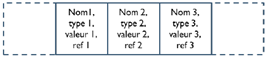
\includegraphics[height=0.08\textwidth]{images/pile2.png}
\end{center}

Suivant la valeur, le cadre peut s'étendre sur un grand nombre de bits.\\
Pour les types Python non mutables (int, float, str, tuple) il est possible de considérer que les données sont juxtaposées car il est possible de connaître la taille de chaque variable lors de l'affectation.\\
Pour les types mutables (comme les listes), on ne sait pas à l'avance combien d'emplacements mémoire vont être nécessaires car on peut ajouter des données à une même liste de façon indéfinie. Ce sont des structures de taille variable (dynamique) et linéaire.\\
Dans beaucoup de langages de programmation, les listes sont de type array (tableau) des structures de taille fixe (statique) :
\begin{itemize}
\item un nombre de cases fixées à l'avance par l'utilisateur ;
\item des cases qui sont toutes du même type ;
\item un accès aux cases se faisant théoriquement à coût constant (O(1)).
\end{itemize}
En Python, ce n'est pas le cas ce qui rend très aisé la gestion des piles et des files.

\subsection{Importance des piles en informatique}

Les piles sont les objets les plus fondamentaux en informatique.\\
L'insertion et la suppression se font toujours du même côté, le fond n'est jamais accessible, seul le sommet est accessible.\\


\begin{minipage}[c]{0.78\linewidth}
	\begin{itemize}
	\item mémorisation des pages visitées dans un navigateur web, l'adresse de chaque nouvelle page visitée est empilée et l'utilisateur dés-empile l'adresse de la page précédente en cliquant sur précédente ;
	\item gestion des environnements d'exécution des fonctions en particulier récursives ;
	\item gestion des expressions arithmétiques de la forme $5 \times (3-6)+(1+7) \times 12$ sans parenthèse (notation polonaise inversée) ;
	\item retour en arrière dans des logiciels de création de document ou des logiciels de jeux avec \texttt{Ctrl z} ;
	\item pour construire le parcours d'un graphe \textbf{en profondeur}.
	\end{itemize}
\end{minipage}
\hfill%
\begin{minipage}[c]{0.2\linewidth}
	\begin{center}
	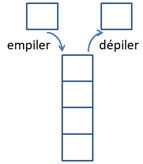
\includegraphics[width=3cm]{images/pile1.png}
	\end{center}
\end{minipage}


\subsection{Importance des files en informatique}

L'insertion d'un élément se fait par le sommet et la suppression se fait par le fond.

\begin{itemize}
\item une file d'attente ;
\item les mémoires tampons (buffers) ;
\item les systèmes d'exploitation multitâches qui
répartissent le temps-machine entre différentes
tâches ;
\item les serveurs d'impression qui traitent les requêtes
dans l'ordre d'arrivée ;
\item pour construire le parcours d'un graphe \textbf{en largeur}.
\end{itemize}


\subsection{Implémentation des piles}

L'implémenter des piles se fait généralement à partir de listes (parfois des tableaux et dans ce cas là, la taille est imposée).\\
Chacun des éléments de la pile peut être un objet de type différent. Le coût des opérations suivantes est constant.\\
Il y a quatre opérateurs définis pour les piles à partir desquels toutes les manipulations sont possibles.

\begin{lstlisting}
# opération 1 : créer une pile vide
pile=[] # cout constant

# opération 2 : vérifier que la pile est vide
len(pile)==0 # cout constant

# opération 3 : empiler un élément v dans la pile (v est forcément ajouté en dernière place)
pile.append(v) # cout constant

# opération 4 : dépiler une pile (c'est forcément le dernier élément qui est enlevé)
sommet=pile.pop() # cout constant
\end{lstlisting}


\subsection{Implémentation des files avec le module deque}

Les deques (se prononce \og\,dèque\,\fg{}, de l'anglais \emph{deque} pour \emph{double-ended queue}, littéralement \og\,file à deux bouts\,\fg{}) sont accessibles grâce à la bibliothèque \texttt{collections}. Comme son nom l'indique, elle optimise l'ajout et le retrait d'élément par les 2~bouts.\\
Chacun des éléments de la file peut être un objet de type différent.\\
Il y a quatre opérateurs à coût constant définis pour les files à partir desquels toutes les manipulations sont possibles.

\begin{lstlisting}
from collections import deque

# opération 1 : créer une file vide
file=deque()

# opération 2 : vérifier que la file est vide
len(file)==0

# opération 3 : enfiler un élément v dans la file (v est ajouté a droite)
file.append(v) # on pourrait enfiler v a gauche file.appendleft(v)

# opération 4 : défiler une file (c'est le premier élément qui est enlevé, celui a gauche)
sortie=file.popleft() # on pourrait défiler a droite sortie=file.pop()

# opérations utiles liées a deque
# vider une file
file.clear()
# copier une file
F=file.copy()
\end{lstlisting}

Les piles sont des listes qui peuvent être de longueur "illimitée" même avec le module \texttt{deque}. Pour les files, il est possible d'imposer une longueur en fixant \texttt{maxlen}. Dans ce cas là, si la file est pleine par ajout d'éléments alors elle se vide à l'autre extrémité.


\begin{lstlisting}
from collections import deque

file=deque(maxlen=6)
for i in range(5):
    file.append(i)
print (file)
for j in ['pts1','pts2','pt','ptstar']:
    file.append(j)
print (file)
\end{lstlisting}

\begin{pythonshell}
deque([0, 1, 2, 3, 4], maxlen=6)  \# le 6e élément n'est pas défini\\
deque([3, 4, 'pts1', 'pts2', 'pt', 'ptstar'], maxlen=6)
\end{pythonshell}




%\begin{figure}[h]
%    \begin{minipage}[c]{.32\linewidth}
%        \centering
%        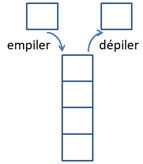
\includegraphics[height=0.7\textwidth]{images/pile1.png}
%        \caption{Plan de la ville avec les ponts}
%        \label{image1}
%    \end{minipage}
%    \hfill%
%    \begin{minipage}[c]{.32\linewidth}
%        \centering
%        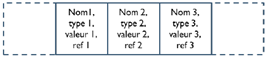
\includegraphics[height=0.7\textwidth]{images/pile2.png}
%        \caption{Représentation schématisée vue du dessus}
%    \end{minipage}
%    \hfill%
%    \begin{minipage}[c]{.32\linewidth}
%        \centering
%        
\includegraphics[height=0.7\textwidth]{images/pile3}
%        \caption{Représentation sous forme de graphe}
%    \end{minipage}
%\end{figure}


\section{Exemples d'utilisation des deques}

\subsection{Utilisation d'une pile pour la conversion de base}

On a les 2 fonctions suivantes pour obtenir la conversion d'un entier vers une liste de bits et inversement~: 

\begin{lstlisting}
def convToBinary(n):
    q=n
    L=[]
    while q!=0:
        L.append(q%2)
        q//=2
    return L

def convFromBinary(L):
    n=0
    while not len(L)==0:
        n*=2
        n+=L.pop()
    return n
\end{lstlisting}

\cache{   
convToBinary(10)=[0, 1, 0, 1]\\
convFromBinary([0, 1, 0, 1])=10}

Le fonctionnement est bon et à coût minimum, mais la liste des chiffres n'est pas dans un ordre de lecture satisfaisant (lecture de droite à gauche au lieu de gauche à droite). 

Proposer des modifications utilisant une deque à la place d'une liste afin de régler ce souci sans détériorer la complexité.
   
\begin{python}
\Cache{
from collections import deque\\
def convToBinary2(n):\\
\indente q=n\\
\indente     L=deque()\\
\indente     while q!=0:\\
\indente \indente         L.appendleft(q\%2)\\
\indente \indente         q//=2\\
\indente     return L\\
def convFromBinary2(L):\\
\indente     n=0\\
\indente     while not len(L)==0:\\
\indente \indente         n*=2\\
\indente \indente         n+=L.popleft()\\
\indente     return n}
\end{python}
\cache{
\# convToBinary2(11)= deque([1, 0, 1, 1])\\
\# convFromBinary2(deque([1, 0, 1, 1]))= 11}

\subsection{Utilisation d'une file pour faire une permutation circulaire}

On souhaite utiliser une file pour faire une permutation circulaire d'un cran. La fonction \texttt{perm\_circ(f)}, doit renvoyer f qui a subie une permutation circulaire (si \texttt{[1, 2, 3, 4]} est mis en entrée, on souhaite voir ressortir \texttt{deque([4, 1, 2, 3])}).

\begin{python}
\Cache{
def perm\_circ(L):\\
\indente     f=deque(L)\\
\indente     sommet=f.pop()\\
\indente     f.appendleft(sommet)\\
\indente     return f}
\end{python}

\subsection{La parenthèse inattendue}

Dans cet exercice, on souhaite savoir si une chaîne de caractères est bien parenthésée ou non. 
Une chaîne bien parenthésée est une chaîne vide ou bien la concaténation de chaînes bien parenthésées.


\begin{exes}
Chaînes bien parenthésées :
\begin{itemize}
\item \texttt{"()"},\texttt{"()()"},\texttt{"(())"} et \texttt{"(()())"}.
\end{itemize}
Chaînes mal parenthésées :
\begin{itemize}
\item \texttt{")("},\texttt{"(("},\texttt{"(()"} et \texttt{"())"}.
\end{itemize}
\end{exes} 

\begin{qexo}
\'Ecrire la fonction \texttt{parentheses(chaine:str)->bool} prenant en argument une chaîne de caractères constituée uniquement de parenthèses et affichant les couples d'indice parenthèse ouvrante, parenthèse fermante. Cette fonction renvoie \texttt{True} si la chaîne est bien parenthésée et \texttt{False} sinon.
\end{qexo} 

\begin{pythonshell}
\invite parentheses('(())()')\\
(1, 2)\\
(0, 3)\\
(4, 5)
\end{pythonshell}


\vfill
\textbf{Références :}\\
T. Kovaltchouk, \textit{Informatique Commune PCSI}, Reims\\
UPSTI, \textit{Informatique Commune}



\newpage
\renewcommand{\contentsname}{Plan du cours}
\tableofcontents


\end{document}
